\section{Manual Operation}
The \productNumber ~\productName ~features two operation modes. It can be either operated using the manual user interface or remote controlled by a computer. In this section the manual operation of the device is explained.
\subsection{Menu structure}
After turning on the \productName ~it comes up with its start screen. Turning the rotary encoder serves to scroll through the menus (see figure~\ref{main_menu}). Pressing the rotary encoder enters the selected menu. Pressing the menu-escape-button leaves the menu again.

\tikzstyle{menu_style} = [rectangle, rounded corners, minimum width=3cm, minimum height=1cm,text centered, draw=black]
\tikzstyle{arrow} = [thick,<->,>=latex]
\def \textWidth {7cm}

\begin{figure}[H]
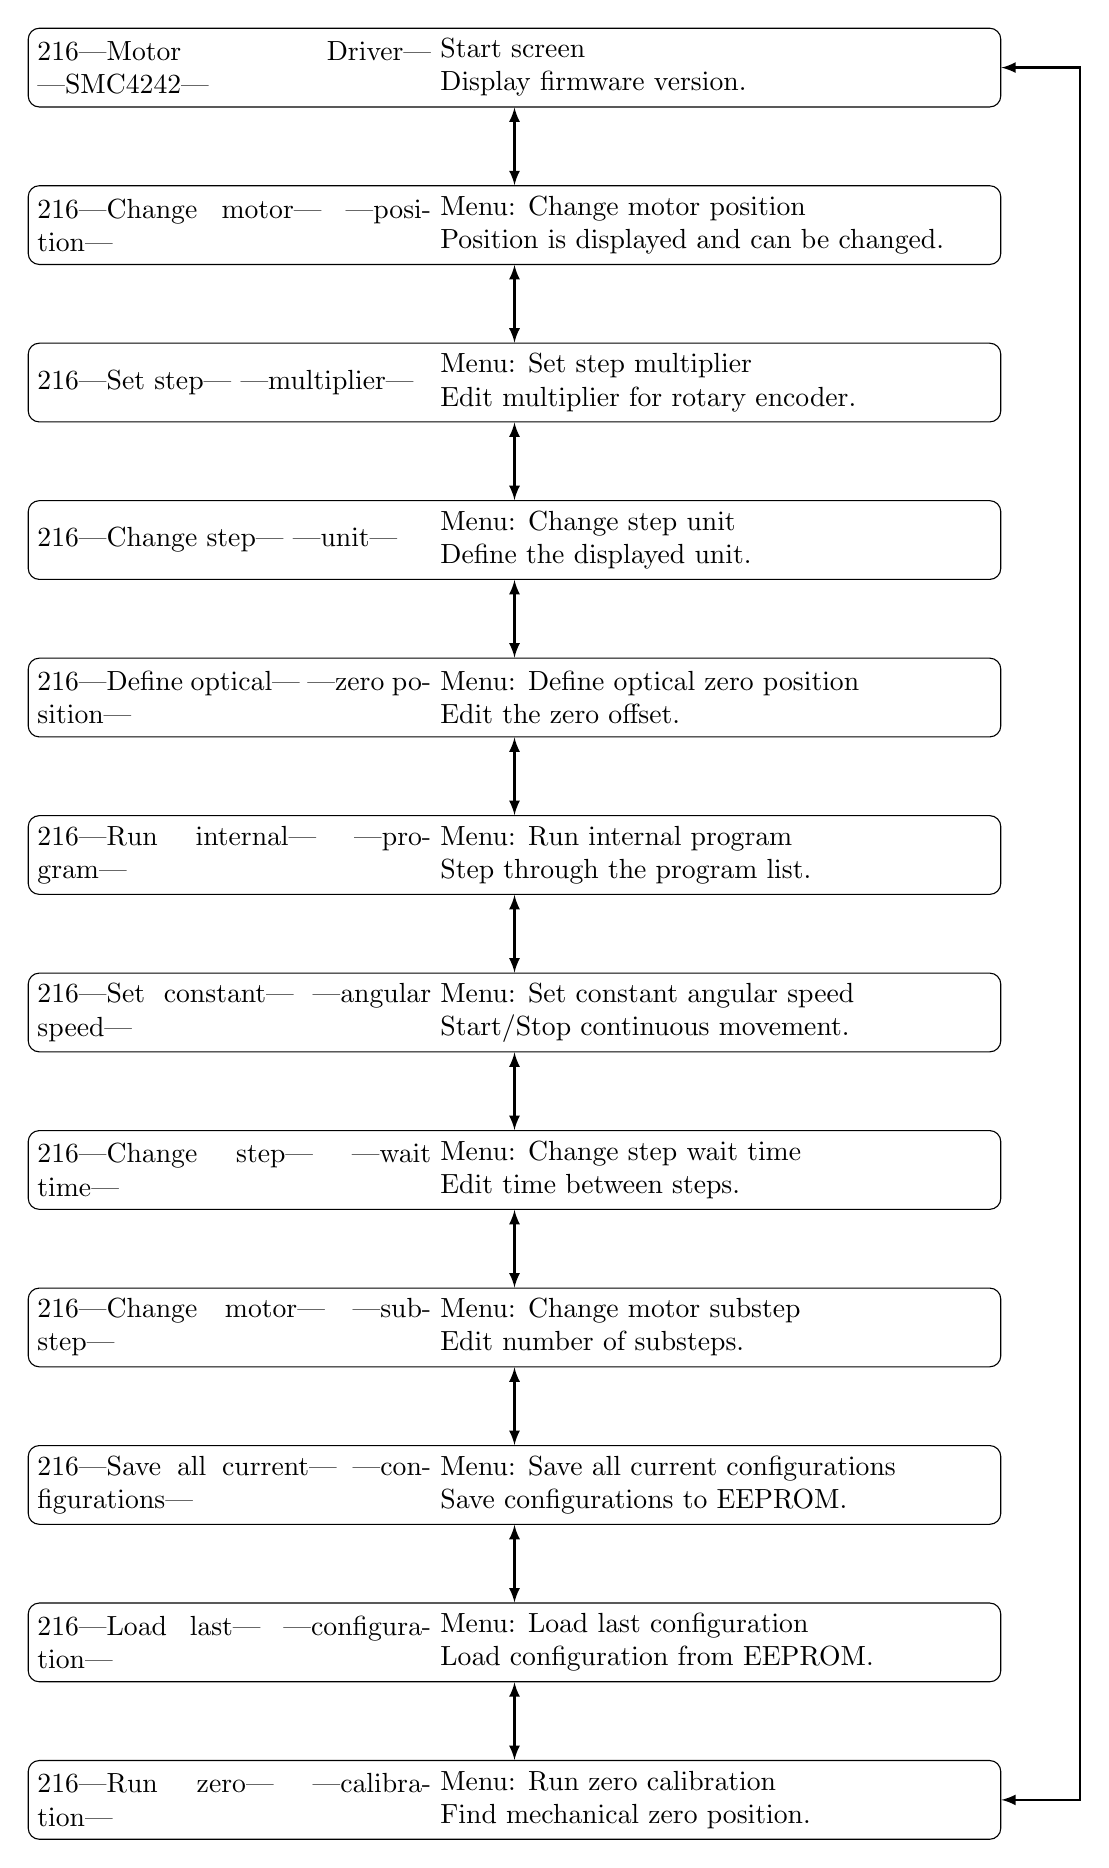
\begin{tikzpicture}[node distance=2cm]
\node (start) [menu_style] {
\begin{minipage}[h]{5cm}
\LCD{2}{16}|Motor Driver|
|SMC4242|
\end{minipage}
 \hfill
\begin{minipage}[h]{\textWidth}
Start screen\\
Display firmware version.
\end{minipage}
};

\node (motor_pos) [menu_style, below of=start] {
\begin{minipage}[h]{5cm}
\LCD{2}{16}|Change motor|
|position|
\end{minipage}
 \hfill
\begin{minipage}[h]{\textWidth}
Menu: Change motor position\\
Position is displayed and can be changed.
\end{minipage}
};

\node (step_multiplier) [menu_style, below of=motor_pos] {
\begin{minipage}[h]{5cm}
\LCD{2}{16}|Set step|
|multiplier|
\end{minipage}
 \hfill
\begin{minipage}[h]{\textWidth}
Menu: Set step multiplier\\
Edit multiplier for rotary encoder.
\end{minipage}
};

\node (step_unit) [menu_style, below of=step_multiplier] {
\begin{minipage}[h]{5cm}
\LCD{2}{16}|Change step|
|unit|
\end{minipage}
 \hfill
\begin{minipage}[h]{\textWidth}
Menu: Change step unit\\
Define the displayed unit.
\end{minipage}
};

\node (optical_zero) [menu_style, below of=step_unit] {
\begin{minipage}[h]{5cm}
\LCD{2}{16}|Define optical|
|zero position|
\end{minipage}
 \hfill
\begin{minipage}[h]{\textWidth}
Menu: Define optical zero position\\
Edit the zero offset.
\end{minipage}
};

\node (internal_prog) [menu_style, below of=optical_zero] {
\begin{minipage}[h]{5cm}
\LCD{2}{16}|Run internal|
|program|
\end{minipage}
 \hfill
\begin{minipage}[h]{\textWidth}
Menu: Run internal program\\
Step through the program list.
\end{minipage}
};

\node (const_speed) [menu_style, below of=internal_prog] {
\begin{minipage}[h]{5cm}
\LCD{2}{16}|Set constant|
|angular speed|
\end{minipage}
 \hfill
\begin{minipage}[h]{\textWidth}
Menu: Set constant angular speed\\
Start/Stop continuous movement.
\end{minipage}
};

\node (step_wait_time) [menu_style, below of=const_speed] {
\begin{minipage}[h]{5cm}
\LCD{2}{16}|Change step|
|wait time|
\end{minipage}
 \hfill
\begin{minipage}[h]{\textWidth}
Menu: Change step wait time\\
Edit time between steps.
\end{minipage}
};

\node (substep) [menu_style, below of=step_wait_time] {
\begin{minipage}[h]{5cm}
\LCD{2}{16}|Change motor|
|substep|
\end{minipage}
 \hfill
\begin{minipage}[h]{\textWidth}
Menu: Change motor substep\\
Edit number of substeps.
\end{minipage}
};

%----------------------------------------------------------------------
% zusaetzliche Menues hier einfuegen!
%----------------------------------------------------------------------

\node (save) [menu_style, below of=substep] {
\begin{minipage}[h]{5cm}
\LCD{2}{16}|Save all current|
|configurations|
\end{minipage}
 \hfill
\begin{minipage}[h]{\textWidth}
Menu: Save all current configurations\\
Save configurations to EEPROM.
\end{minipage}
};

\node (load) [menu_style, below of=save] {
\begin{minipage}[h]{5cm}
\LCD{2}{16}|Load last|
|configuration|
\end{minipage}
 \hfill
\begin{minipage}[h]{\textWidth}
Menu: Load last configuration\\
Load configuration from EEPROM.
\end{minipage}
};

\node (zero_cal) [menu_style, below of=load] {
\begin{minipage}[h]{5cm}
\LCD{2}{16}|Run zero|
|calibration|
\end{minipage}
 \hfill
\begin{minipage}[h]{\textWidth}
Menu: Run zero calibration\\
Find mechanical zero position.
\end{minipage}
};

\draw [arrow] (start) -- (motor_pos);
\draw [arrow] (motor_pos) -- (step_multiplier);
\draw [arrow] (step_multiplier) -- (step_unit);
\draw [arrow] (step_unit) -- (optical_zero);
\draw [arrow] (optical_zero) -- (internal_prog);
\draw [arrow] (internal_prog) -- (const_speed);
\draw [arrow] (const_speed) -- (step_wait_time);
\draw [arrow] (step_wait_time) -- (substep);
%------------------------------------------
\draw [arrow] (substep) -- (save);
\draw [arrow] (save) -- (load);
\draw [arrow] (load) -- (zero_cal);
\draw [arrow] (zero_cal.east) -- +(1,0) |- (start.east);
\end{tikzpicture}
\caption[Overview of the available menus.]{Overview of the available menus. By rotating the rotary encoder one can navigate through the list of menus as indicated by the arrows.}
\label{main_menu}
\end{figure}

\subsubsection{Display structure}
In almost every menu four values are displayed. Depending on the previously selected menu the values correspond to different quantities. Where\\
the upper left value accompanies to Motor 0,\\
the upper right value accompanies to Motor 1,\\
the lower left value accompanies to Motor 2 and\\
the lower right value accompanies to Motor 3.

\subsubsection{Motor selection}
To select a motor there are four buttons. Motor selection can solely be done in an entered menu. To select a motor, press the respective motor-selection button. A selected motor is signed with an arrow on the display. Pressing the selection-button again deselects the motor. Once a motor is selected its appropriate value can be changed by turning the rotary encoder. By leaving a menu without motor deselection the selected motor(s) stay selected in an other menu.

\subsubsection{Start screen}
When entering the menu behind the start screen, the firmware version will be displayed.
\LCD{2}{16}||
|v1.3|

\subsubsection{Menu: Change motor position}
\label{menu_motor_pos}
In this menu the current motor positions are displayed and can be changed by the operator. The default display unit is degree. The position of a selected motor can be changed by turning the rotary encoder. Default steps for different units are:
\begin{itemize}
\item $1\degree$ if unit is degree
\item $0.125 \cdot \pi$ if unit is radian
\item 1 step if unit is steps
\end{itemize}

\LCD{2}{16}|{rarrow}0.0{pi}   {rarrow}0.0|
           |{rarrow}0st    {rarrow}0.0|

When pressing the rotary encoder in this menu one enters the fast moving mode. Pressing the rotary encoder again leaves the fast mode. The fast moving mode can be noticed by another marking arrow. Default steps in fast mode are:
\begin{itemize}
\item $10\degree$ if unit is degree
\item $0.125 \cdot \pi$ if unit is radian
\item 100 steps if unit is steps
\end{itemize}

\LCD{2}{16}|>0.0   >0.0||>0.0   >0.0|

\subsubsection{Menu: Set step multiplier}
In this menu one can adjust a step multiplier. The step multiplier is applied if the step unit is degree or radian. The standard value is 1.0. If the step multiplier differs from 1.0 the corresponding motor will rotate more or less steps with each rotation of the rotary encoder.\\
For example: if the step multiplier for motor 0 is 1.0 and the step multiplier for motor 2 is 4.0, motor 2 will move four times more steps than motor 0 when changing the motors positions. Negative values are allowed as well. This will result in counter direction movements.

\LCD{2}{16}|{rarrow}1.0x   {rarrow}-0.5x|
|{rarrow}2.0x    1.0x|

\subsubsection{Menu: Change step unit}
In this menu one can choose the unit of the displayed position. There are three possible choices for each motor:
\begin{itemize}
\item degree
\item radian
\item step
\end{itemize}

\LCD{2}{16}|{rarrow}radian {rarrow}degree|
|{rarrow}step    degree|

\subsubsection{Menu: Define optical zero position}
In this menu one can define the optical zero position. This is necessary due to a mostly unknown placement of the optical element mounted to the motor. Here one can once adjust the desired optical zero position manually. The optical zero position is always defined in steps. In this menu there is also a fast mode available (please refer to \ref{menu_motor_pos} for details about the fast mode). After adjustment it is recommended to save this configuration (see \ref{menu_save}).
When performing a zero calibration, as explained in \ref{menu_zero_cal}, the zero position will be the defined optical zero position.

\LCD{2}{16}|{rarrow}0st     0st|
| 0st     0st|

\subsubsection{Menu: Run internal program}
This menu allows the user to step through the internal program list. This function is available only if a program has previously been defined (see \ref{section_instruction_set}).

\LCD{2}{16}|Program running|
|Step 0|

\subsubsection{Menu: Set constant angular speed}
Here the motors can be set into an infinite moving state in clockwise (CW) or counter clockwise (CCW) direction. To get the motors moving with different velocities one needs to change the wait times between two steps (see \ref{menu_step_wait_time}).

\LCD{2}{16}|{rarrow}CW     {rarrow}CCW|
| STOP    STOP|

\subsubsection{Menu: Change step wait time}
\label{menu_step_wait_time}
Here the wait time between two steps can be changed. This results in faster or slower motor movements. The default value is 3 milliseconds. We do not recommend to use shorter wait times, even if this works.

\LCD{2}{16}|{rarrow}3 ms   {rarrow}3 ms|
|{rarrow}3 ms    3 ms|

\subsubsection{Menu: Change motor substeps}
In this menu one can change the motor substeps. Possible values are 1, 2, 4, 8, 16 or 32.

\LCD{2}{16}|{rarrow}1      {rarrow}2|
| 4      {rarrow}8|

%----------------------------------------------------------------------
% zusaetzliche Menues hier einfuegen!
%----------------------------------------------------------------------

\subsubsection{Menu: Save current configurations}
\label{menu_save}
To save the current \productName ~configurations enter this menu and turn the rotary encoder in any direction. The menu will be automatically leaved when saving is finished.\\
Note: The configurations for all motors will be saved.

\LCD{2}{16}|Save all current|
|configurations|

\subsubsection{Menu: Load last configuration}
To load the last saved \productName ~configurations enter this menu and turn the rotary encoder in any direction. The menu will be leaved automatically when loading has
finished.\\
Note: The last saved configuration is loaded automatically when powering on the \productName.\\
Note: There is just one memory space for a configuration.

\LCD{2}{16}|Load all saved|
|configurations|

\subsubsection{Menu: Run zero calibration}
\label{menu_zero_cal}
Here one can calibrate the motor zero position for each motor. To perform a zero calibration select the motors to be calibrated and turn the rotary encoder. Note, that during zero calibration no actions can be done on the device, even serial commands will not be accepted. The zero calibration will automatically deselect a motor when its calibration is finished. The zero calibration menu will be automatically leaved when calibration is finished.

\LCD{2}{16}|{rarrow}Mot 0  {rarrow}Mot 1|
| Mot 2   Mot 3|











\newpage
